\section{De-amortized constructions:LSDd}\label{sec:de-amortized}
Although \SDa provides a clean way to transform a static SE scheme to a dynamic one, its drawback is that it has amortized update cost. In the worst case an update may require rebuilding an index of size $N$ at once. 
Figure {app-fig:update} illustrates the above weakness of schemes with amortized update cost. 
In this section, we construct I/O efficient DSE schemes with de-amortized updates and with forward and backward privacy. 
Our starting point is the de-amortization strategy that Demertzis et al.~\cite{SDa} proposed for \SDa, called  \SDd\ (which is tailored on \PiBas \cite{cash2014dynamic}; {pseudocode of \PiBas\ can be found in the extended version}.
In this work, we introduce \LSDd, which is simpler than \SDd\ and separates the static-to-dynamic transformation from the underlying static SE scheme. 
We highlight that \LSDd\ is not a compiler; it is specifically tailored for certain schemes, namely \OneChoice, \TwoChoice, and \NlogN\ schemes. 
We present \LSDd\ primarily as a framework for the sake of clarity and concise presentation. 
Below, we explain the new \LSDd: \label{subsec:deamortized}

\begin{algorithm}
  %\caption{Voting Protocol}
  \caption{$(K,\sigma;EDB) \gets \setup(\lambda, N)$}
  \label{alg:setup}
  \begin{algorithmic}[1]
  \State $\ell \gets  \lceil{\log N}\rceil$;\quad 
$upd_{cnt} \leftarrow 0$;
\State Set matrix $P$ of size $(\ell+1){\cdot} 4$
\State $k_{rnd} \gets \RND.\keyGen(1^\lambda)$
\State $\sigma \leftarrow \{upd_{cnt}\}$ and $K \gets (k_{rnd},P)$
\State Initialize an empty $EDB$
\State \Return $EDB$ to Server and $(K,\sigma)$ to the Client
  \end{algorithmic}
\end{algorithm}

\begin{algorithm}
\caption{$(K,\sigma;EDB) \gets \setup(\lambda, N)$}
\begin{algorithmic}[1]
\State $\ell \gets  \lceil{\log N}\rceil$;\quad 
$upd_{cnt} \leftarrow 0$;
\State Set matrix $P$ of size $(\ell+1){\cdot} 4$
\State $k_{rnd} \gets \RND.\keyGen(1^\lambda)$
\State $\sigma \leftarrow \{upd_{cnt}\}$ and $K \gets (k_{rnd},P)$
\State Initialize an empty $EDB$
\State \Return $EDB$ to Server and $(K,\sigma)$ to the Client
%\State \Return $(K,\sigma)$ to the Client
\end{algorithmic}
\end{algorithm}


\begin{figure}
\begin{mdframed}	
  %\begin{multicols}{2}
 \underline{$(K,\sigma;EDB) \gets \setup(\lambda, N)$}
\begin{algorithmic}[1]
\State $\ell \gets  \lceil{\log N}\rceil$;\quad 
$upd_{cnt} \leftarrow 0$;
\State Set matrix $P$ of size $(\ell+1){\cdot} 4$
\State $k_{rnd} \gets \RND.\keyGen(1^\lambda)$
\State $\sigma \leftarrow \{upd_{cnt}\}$ and $K \gets (k_{rnd},P)$
\State Initialize an empty $EDB$
\State \Return $EDB$ to Server and $(K,\sigma)$ to the Client
%\State \Return $(K,\sigma)$ to the Client
\end{algorithmic}

\underline{$DB(w) \leftrightarrow {\Search}(K,\Gamma, q,\sigma ; EDB)$}
			%\underline{$\textsf{Search}(st_{\mathcal{C}},w, L)$}
			\begin{algorithmic}[1]
				%\State Parse the array of maps $EDB$ as set of indexes $L$; $\sigma$ as set of states $st$; K as a vector of secret keys ${\sf vec\_key}$ and compute $\ell = \lfloor \log N \rfloor$.
				%\State Parse state $st_{\mathcal{C}}$ as $(\lambda,{\sf vec\_key}, N)$. Compute $\ell = \lfloor \log N \rfloor$.
				\item[Client $\leftrightarrow$ Server:]
				\State $\mathcal{X}\leftarrow\emptyset$
				\For{$i=\ell \cdots 0$}
				\If {${\OLDEST}_i.\Ind \neq \emptyset$} 
    %\tpurp{the definition of $\Sigma.\Search$ does not have $2^i$ as a parameter, but we need it here, \Search also takes the static scheme $\Sigma'$ as an input parameter, should we change the definition ??}
				\State \hskip-0.7em$\mathcal{X} \leftarrow \mathcal{X} \; \cup$ {$\Gamma$.\Search}($K[i][0], q,\sigma;{\OLDEST}_i$)
				\EndIf
				\If {${\OLDER}_i.\Ind \neq \emptyset$}
				\State \hskip-0.7em$\mathcal{X}$ $\leftarrow$ $\mathcal{X}$ $\cup$ {$\Gamma$.\Search}($K[i][1],q,\sigma; {\OLDER}_i$)
				\EndIf
				\If {${\OLD}_i.\Ind \neq \emptyset$}
				\State \hskip-0.7em$\mathcal{X}$ $\leftarrow$ $\mathcal{X}$ $\cup$ {$\Gamma$.\Search}($K[i][2], q,\sigma;{\OLD}_i$)
				\EndIf
				\EndFor
				\item[Client:]
				%\State Decrypt entries of $\mathcal{X}$ with $K$ parse them as $(id,op)$
				\State $DB(w)\leftarrow\{id\; | \; (w,id,add)\in \mathcal{X} \land (w,id,del) \not\in \mathcal{X}\}$
				%\State \textbf{return} $(\mathcal{X},st_{\mathcal{C}}',\mathcal{I}')$.
			\end{algorithmic}
%\end{multicols}
\end{mdframed}
%\caption{\SDd,\LSDd: from {$\Gamma$=(\keyGen, \Setup, \Search)} to DSE (de-amortized version).}
\label{fig:SSEtoDSE1}
\end{figure}

\newcommand{\var}[1]{\text{\texttt{#1}}}
\newcommand{\func}[1]{\text{\textsl{#1}}}
\newcounter{phase}[algorithm]
\newlength{\phaserulewidth}
\newcommand{\setphaserulewidth}{\setlength{\phaserulewidth}}
\newcommand{\phase}[1]{%
  \vspace{-1.25ex}
  % Top phase rule
  \Statex\leavevmode\llap{\rule{\dimexpr\labelwidth+\labelsep}{\phaserulewidth}}\rule{\linewidth}{\phaserulewidth}
  \Statex\strut\textit{$\triangleright$ #1 }% Phase text
  % Bottom phase rule
  \vspace{-1.25ex}\Statex\leavevmode\llap{\rule{\dimexpr\labelwidth+\labelsep}{\phaserulewidth}}\rule{\linewidth}{\phaserulewidth}}
\setphaserulewidth{.7pt}

\begin{algorithm}
  \caption{Voting Protocol}
  \label{alg:phoenix-voting}
  \begin{algorithmic}[1]
    \phase{\textbf{as a replica k}} \\
    When replica \texttt{j} is suspected\\
    \hskip 1em broadcast $\langle VOTE, j, getLatestDec(\texttt{DecLog})$, \O $\rangle_{\sigma_{k}}$\\
  \vspace{0.1cm}
    When replica \texttt{j} is detected with Proof \\
    \hskip 1em broadcast $\langle VOTE, j, getLatestDec(\texttt{DecLog}), Proof \rangle_{\sigma_{k}}$\\
  \vspace{0.1cm}
    When received m : $\langle VOTE, j, Cert, Proof \rangle_{\sigma_{i}}$ from
    replica \texttt{i}\\
    \hskip 1em \textbf{if} \texttt{i} in \texttt{Conf} $\land$ \texttt{m.j} in
    \texttt{Conf} $\land$ isValidCert(\texttt{m.Cert})\\
\end{algorithmic}
\end{algorithm}

\begin{figure}%[!h]
%\begin{mdframed}	
\underline {$(K, \sigma; EDB) \leftrightarrow$ {\texttt{Update}$(K,(w,id,op),\Gamma,\sigma;EDB)$}}
%\underline {\sf Update$(op,w,id,st_{\mathcal{C}})$}
\begin{algorithmic}[1]
\item[Client $\leftrightarrow$ Server:]
\State Parse $K$ as $(k_{rnd},P)$ \Comment{$k_{rnd}$ is encryption key, $P$ is an array of PRF keys}
\For{$i=\ell, \dots, 1$}
\If {${\OLDEST}_{i-1}.\Ind \neq \emptyset \land {\sf OLDER}_{i-1}.\Ind \neq \emptyset$} \Comment{$\Gamma$ is \{\PiBas,\OneChoice,\TwoChoice,\NlogN\}}
\State{Execute the next $\gamma$ steps of $\Gamma$.\omerge$(K,\sigma,\OLDEST_{i-1},\OLDER_{i-1})$ and update $\NEW_i$} \label{alg:ssetodse1} 
\If {${\sf NEW}_i.\Ind$ is full}\label{sddalg:newfull}\Comment{Client can deduce this from $upd_{cnt}$}
\State Server sets ${\OLDEST}_{i-1}\leftarrow {\OLD}_{i-1}$  and ${\OLDER}_{i-1} \leftarrow \emptyset$ \label{sddalg:oldmove}
\If {${\OLDEST}_{i}.\Ind = \emptyset$} server sets ${\OLDEST}_{i} \leftarrow {\NEW}_{i}$ and client sets $P[i][0] \leftarrow P[i][3]$ \label{sddalg:newmove1}
\ElsIf {${\OLDER}_{i}.\Ind = \emptyset$} server sets ${\OLDER}_{i} \leftarrow {\NEW}_{i}$ and client sets $P[i][1] \leftarrow P[i][3]$ \label{sddalg:newmove2}
\Else {} server sets ${\OLD}_{i} \leftarrow {\NEW}_{i}$ and client sets $P[i][2] \leftarrow P[i][3]$ \label{sddalg:newmove3}
\EndIf
\State Client sets $P[i][3] \leftarrow$ {$\Gamma$}.{\texttt{KeyGen}}$(1^\lambda)$ \label{sddalg:keygen}
\EndIf
\EndIf
\EndFor
\State Client sets $P[0][3] \leftarrow$ {$\Gamma$}.{\texttt{KeyGen}}$(1^\lambda)$ \label{sddalg:keygen0}
			\State Client runs {$\Gamma$}.\setup($P[0][3]$, $(w,id,op)$) and sends the output to server who stores it as ${\sf NEW}_0$ \label{sddalg:new0full}
			\If {${\sf OLDEST}_0.\Ind = \emptyset$} server sets ${\sf OLDEST}_0 \leftarrow {\sf NEW}_0$ and client sets  $P[0][0] \leftarrow P[0][3]$ \label{sddalg:new0move2}
			\ElsIf {${\sf OLDER}_0.\Ind = \emptyset$} server sets ${\sf OLDER}_0 \leftarrow {\sf NEW}_0$ and client sets  $P[0][1] \leftarrow P[0][3]$ \label{sddalg:new0move3}
			\Else {} Server sets ${\sf OLD}_0 \leftarrow {\sf NEW}_0$ and client sets  $P[0][2] \leftarrow P[0][3]$ \label{sddalg:new0move3}
			\EndIf
			\State Client sets $upd_{cnt} \leftarrow upd_{cnt}+1$
\State \Return $EDB$ to Server and $(K,\sigma)$ to Client
			%\State Update $K, \sigma, EDB$ accordingly.
			%\State \textbf{return} $(K,\sigma,EDB)$.
		\end{algorithmic}
	%\end{mdframed}
	\caption{\SDd/\LSDd: from {$\Gamma$=(\keyGen, \Setup, \Search)} to DSE (de-amortized version).}
	\label{fig:SSEtoDSE2}
 %\vspace{-1.2em}
\end{figure}







\smallskip\noindent\textbf{Overview of \textbf{\LSDd[$\cdot$].}}  The main idea of \LSDd[$\cdot$]\ framework is to split  construction steps of index level $i$ over the previous $2^i$ insertions. We use a static SE scheme $\Gamma$=(\keyGen, \Setup, \Search). For dataset size $N$, \LSDd[$\Gamma$]~keeps ${\log N}$ index levels. Every $i$th index level has $4$ indexes (a.k.a. ${\sf NEW}_i$, ${\sf OLD}_i$, ${\sf OLDER}_i$ and ${\sf OLDEST}_i$); every index stores $2^i$ real entires. %An index in level $i$ stores $2^i$ entries and it is built using the static SE scheme $\Gamma$. 
The \LSDd[$\Gamma$].\texttt{Search} simply queries the ${\sf OLD_i}$, ${\sf OLDER_i}$ and ${\sf OLDEST_i}$ indexes by individually calling $\Gamma$.\texttt{Search} for all ${\log N}$ levels as a black box (see \texttt{Search} in Figure \ref{fig:SSEtoDSE1}). Index ${\sf NEW}_i$ is used as a temporary buffer for moving elements between levels $i-1$ and $i$ during \LSDd[$\Gamma$].\texttt{Update}.  Below, we explain \LSDd[$\Gamma$].\texttt{Update} in three rules: 

\noindent\underline{(Rule 1):} An update for $(w,id,op)$ (insert or delete) is performed by creating  ${\sf NEW}_0$ (i.e. an encrypted index \NEW$_0$.\Ind\ and an encrypted dictionary \NEW$_0$.\Dict)
%using the \texttt{KeyGen} and \texttt{Setup} of %the used static SE scheme $\Gamma$, i.e., 
by calling $\Gamma$.\texttt{KeyGen} and $\Gamma$.\texttt{Setup} 
in a black-box manner (see lines \ref{sddalg:keygen0}-\ref{sddalg:new0full} in Figure \ref{fig:SSEtoDSE2})---this instantly triggers the next rule. 

\noindent\underline{(Rule 2):} If ${\sf NEW}_i.\Ind$ is full, then ${\sf NEW}_i$ is moved\footnote{$\OLDEST_i$$\gets$$\NEW_i$ is syntactic sugar for $(\OLDEST_i.\Ind$, $\OLDEST.\Dict)$ $\gets$$(\NEW_i.\Ind$, $\NEW_i.\Dict)$} to the oldest $empty$ index among $\OLDEST_{i}$,$\OLDER_{i}$, and $\OLD_{i}$ (see lines \ref{sddalg:new0move2}-\ref{sddalg:new0move3} for level 0 and lines \ref{sddalg:newfull}-\ref{sddalg:keygen} for level $i$ in Figure \ref{fig:SSEtoDSE2}). At the end of $2^i$ updates (equivalently moving $2\cdot 2^{i-1}$ elements from level $(i-1)$) ${\sf NEW}_i.\Ind$ becomes full, 
%(i.e. all the elements from ${\sf OLDEST}_{i-1}.\Ind$ and ${\sf OLDER}_{i-1}.\Ind$ have been moved to the next level (using Rule 3)) 
which triggers two actions in level $(i-1)$: ${\sf OLD}_{i-1}$ is moved to ${\sf OLDEST}_{i-1}$, and ${\sf OLDER}_{i-1}$ is set to be empty (line \ref{sddalg:oldmove}). %in Figure \ref{fig:SSEtoDSE2}). 
%Because ${\sf NEW}_i$ is always moved to the oldest available index, ${\sf OLDEST}_i$ is filled before ${\sf OLDER}_i$, and ${\sf OLDER}_i$ is filled before ${\sf OLD}_i$. 
%${\sf NEW}_i$ is used to (merge and) move elements from $(i-1)$th  level to the $i$th level.

\noindent\underline{(Rule 3):} If both ${\OLDER}_{i-1}$$.\Ind$ and ${\OLDEST}_{i-1}$$.\Ind$ are full, %elements from ${\OLDER}$$_{i-1}$$.\Ind$$\cup$${\OLDEST}$$_{i-1}$$.\Ind$ are moved gradually to %$\NEW_i$$.\Ind$---
all the elements of ${\OLDER}_{i-1}.$$\Ind$ $\cup$ ${\OLDEST}_{i-1}.$$\Ind$ are moved to  $\NEW_i$$.\Ind$ over the next $2^i$ updates. Thus, at the end of these $2^i$ updates 
%(equivalently moving $2\cdot 2^{i-1}$ elements) 
${\sf NEW}_i$$.\Ind$ is full, 
and hence ${\sf NEW}_i$ is moved to the oldest $empty$ index in level $i$ using Rule 2.

We demonstrate the above \LSDd[$\Gamma$] rules graphically in Figure \ref{fig:sddFig}. So far, all the actions needed for enforcing the Rules 1 and 2 during \LSDd[$\Gamma$].\texttt{Update} and \LSDd[$\cdot$].\texttt{Search}  are either agnostic to the static SE scheme $\Gamma$, or are using $\Gamma$ in a black-box manner. We mention that the actions needed for \LSDd[$\Gamma$].\keyGen are also agnostic to $\Gamma$ (see Figure \ref{fig:SSEtoDSE1}). 

\neww{We would like to emphasize that up to this point, \LSDd\ is identical to \SDd\cite{SDa}. Below, we detail how \LSDd\ differs from \SDd.} Rule 3 gradually builds $\NEW_i$ by moving elements from ${\sf OLDER}_{i-1}.\Ind$ and ${\sf OLDEST}_{i-1}.\Ind$, i.e. $\Gamma$.\new{\texttt{Setup} for $\NEW_i$ needs to be executed in an incremental fashion. In other words, $\Gamma$.\texttt{Setup} cannot be used as a black-box here. }
To overcome this obstacle, we define a new \emph{oblivious merge} protocol as follows:%\vspace{-3pt}
\begin{align*}
\hspace{-0.1cm}\NEW_i\leftarrow \omerge_i{(K,\sigma,\OLDEST_{i-1}},{\OLDER_{i-1})}
\end{align*}

\new{For each index level $i$, an instance of \emph{oblivious merge} (denoted as \omerge$_i$) needs to be executed.
The \omerge$_i$ protocol takes as input a structure of necessary keys as $K$ (created and maintained from \LSDd[$\cdot$]), client's local state $\sigma$, ${\sf OLDEST}_{i-1}$ and ${\sf OLDER}_{i-1}$, and creates ${\sf NEW}_i$.} We claim that if a static $\Gamma$.\texttt{Setup} can be transformed to an \omerge $_i$\ with the following {three} properties then it can be used in conjunction with the \LSDd{'s} update functionality to de-amortize the corresponding \SDa$[\Gamma]$ construction (maintaining forward and backward privacy). These properties are:
\begin{itemize}
    \item \underline{\textsf{(P1):}} \emph{Obliviousness}---\omerge$_i$\ has to be oblivious---an algorithm/protocol is oblivious iff for any two same-sized  sequence of memory accesses their resulting access patterns are indistinguishable for anyone but the client. In other words,
    %if \omerge$_i$ is oblivious, then 
    we assume the existence of a simulator, \simomerge$_i$, 
    which takes as an input only the size of the $i$th index (i.e. $2^i$) 
    %of ${\sf OLDEST}_{i-1} \cup {\sf OLDER}_{i-1}$ %($2^i$ updates) 
    and is indistinguishable from $\Gamma$.\omerge$_i$ by any \textsf{PPT} adversary 
    (later, we prove that our $\Gamma$.\omerge$_i$ is oblivious for $\Gamma \in \{\OneChoice,\TwoChoice,\NlogN\}$).
    
    
    \item \underline{\textsf{(P2):}} \emph{Input-Output Indistinguishability}---A \textsf{PPT} adversary can recover a "mapping" between the encrypted input entries (contained in ${\sf OLDEST}_{i-1}.\Ind$ and ${\sf OLDER}_{i-1}.\Ind$) and the corresponding output ones (in ${\sf NEW}_{i}.\Ind$) after the execution of \omerge$_i$ only with a negligible advantage. %\tpurp{we discussed that P1 and P2 should be merged, i.e. obliviousness will have two parts, should we ?}
    
    \item \underline{\textsf{(P3):}} \emph{Decomposability}---Given  \omerge$_i$ that requires $s(2^i)$ steps to produce \NEW$_i$, can be decomposed into $s(2^i)/\gamma$  rounds/steps of $\gamma$ work at a time (i.e., per update).
\end{itemize}

We need {\textsf{(P1)}} in order to achieve forward privacy. If \omerge$_i$ is oblivious, then nothing is leaked about the elements that we are moving from level $(i-1)$ to level $i$, i.e., during an individual update/movement the leakage function $\lp^{Updt}$ can be written as: $\mathcal{L}^{Updt}({op},w,{id})=\mathcal{L'}^{Updt}({op},id)$ where $\mathcal{L'}$ is a stateless function. 
%Since \omerge$_i$ is oblivious---it is simulatable by a simulator \simomerge$_i$\ which takes as an input only the size of the inputs and no information about the keywords of the entries which are updated/moved. \tpurp{This line is redundant}
% \todo{4.Explain difference between SDd+Pibas and SDd[PiBas}
{\textsf{(P2)}} is not required for the  security of \LSDd[${\Gamma}$], e.g., 
the original \PiBas-based \LSDd\ in \cite{SDa} does not achieve \textsf{(P2)} (explained later). 
However, we will see that \textsf{(P2)} is byproduct of \textsf{(P1)} when $\Gamma$ is I/O efficient, 
as well as it simplifies the security analysis of our \LSDd[${\Gamma}$] 
(the simulator can use the search simulator of $\Gamma$ in black box). 
%Intuitively, an I/O efficient $\Gamma$ requires to place same keywords close by while 
%moving elements from level $(i-1)$ to level $i$  
%(which contradicts forward privacy at a first glance)---our main observation is that 
%the forward privacy can be achieved in I/O efficient DSE through oblivious updates (i.e., P1).
%\tpurp{the last line is not clear}

Regarding {\textsf{(P3)}}, every algorithm/protocol naturally can be decomposed into instructions (e.g., CPU instructions), or sets of instructions. By maintaining a state locally (e.g. a counter for each $i$th level), and running a set of instructions at a time, we guarantee the correct execution of the algorithm/protocol. 
{\textsf{(P3)}} allowed us to describe \LSDd[$\Gamma$] independent 
to the used static scheme $\Gamma$ and simplify the presentation of 
$\Gamma$.\omerge$_i$. %can be described as an oblivious setup-like algorithm/protocol. 

\new{The original \Update~protocol of \SDd~in \cite{SDa}, which was \PiBas-specific \SDd, 
%\tblue{we use "\PiBas-specific" a lot of times},
achieves properties \textsf{(P1)} and \textsf{(P3)}. We can also transform \PiBas\ 
(and its setup) to an \omerge\ protocol in order to fit to the the new \LSDd[$\cdot$] transformation.   
% For completeness, we provide \PiBas.\omerge\ in Figure \ref{fig:AllPibas} in 
% the Appendix. 
%@@
For completeness, we provide \PiBas.\omerge\ in the extended version. 
Both versions, \SDd\ presented in \cite{SDa} and 
\SDd[\PiBas] fail to achieve {\textsf{(P2)}} 
(i.e. \emph{input-output indistiguishability}).} For moving each input entry $e$ 
(from ${\sf OLDEST}_{i-1}.\Ind \cup {\sf OLDER}_{i-1}.\Ind$)---one by one, it simply does two 
oblivious accesses to an oblivious dictionary, and it performs a "write" in a 
random position in ${\sf NEW}_i$ (using a PRF), i.e.  
the server can see the corresponding chosen positions in {\sf NEW}$_i$. 
\neww{However, the security does not fail since the positions in {\sf NEW}$_i$ 
are chosen randomly. We can also construct \LSDd[PiBas] that achieves all the properties, including (P2). This construction improves the update cost of the original \SDd\ by a logarithmic factor 
%(see Figure \ref{alg:LSDd[PiBas]} in the Appendix for this construction). 
%@@
(the pseudocode provided in the extended version).
The proof has been omitted because it can be derived from the \LSDd\ proof, as it is based on a subset of the computations required by \LSDd. In our experimental evaluation, we refer to this construction as \LSDd[PiBas].}


%\tblue{as locality does not matter in \PiBas} (and \textsf{P1} is achieved). 
%\PiBas.\texttt{setup} is easily decomposable (for $\gamma = O(1)$) into $2^i$ rounds/steps of $\gamma$ work---lines 3-11 in Figure \ref{fig:PibasOmerge} denote the total work for one step/round; in total $2^i$ rounds are needed. 
%Below, we state the security of the forward/backward private DSE \SDd[$\Gamma$], and provide the proof of Theorem \ref{thm:SDd} in Appendix \ref{app:sse}. 

	
\begin{figure}
\centering
\scalebox{0.9}{
\begin{subfigure}[t]{0.2\textwidth} %one
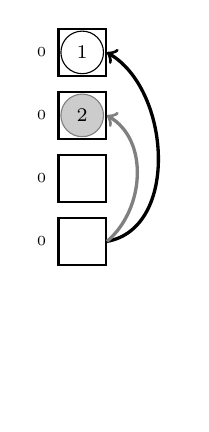
\begin{tikzpicture}
[
textbox/.style={rectangle, draw=white, fill=white,align=center, thick, minimum height=0.5cm},
box1/.style={rectangle, draw=black, fill=white, thick, minimum height=0.6cm, minimum width=2.4cm},
box2/.style={rectangle, draw=black, fill=white, thick, minimum height=0.6cm, minimum width=1.2cm},
box3/.style={rectangle, draw=black, fill=white, thick, minimum height=0.6cm, minimum width=0.6cm},
myarrow1/.style={single arrow, draw=black, fill=black, 
      minimum width = 1mm, single arrow head extend=1mm,
      minimum height=1cm},
myarrow2/.style={single arrow, draw=red, fill=red, 
      minimum width = 1mm, single arrow head extend=1mm,
      minimum height=1.3cm},
myarrow3/.style={single arrow, draw=blue, fill=blue, 
minimum width = 0.09cm, single arrow head extend=0.05cm,
minimum height=0.7cm},
mylabels/.style={text=black, font=\scriptsize},
    every label/.append style={mylabels},
greenball/.style={circle, draw=gray, fill=gray!40, minimum size=1mm},
redball/.style={circle, draw=black, fill=white, minimum size=1mm},
blueball/.style={circle, draw=gray, fill=gray, minimum size=1mm},
]

\node at (0,0) [box3,label={west:$\OLDEST_0$}] (b1)     {};
\node at (0,0) [redball] (g1) {{\scriptsize 1}};
\node at (0,-0.8) [box3,label={west:$\OLDER_0$}] (b2)      {};
\node at (0,-0.8) [greenball] (g2) {{\scriptsize 2}};
\node at (0,-1.6) [box3,label={west:$\OLD_0$}] (b3)               {};
\node at (0,-2.4) [box3,label={west:$\NEW_0$}] (b4)               {};
\node[scale=0.6] at (0.45,-4.3) [textbox] (omap1) {};
\draw [->,black, very thick] (b4.east) to [out=10,in=330] (b1.east) ;
\draw [->,gray,very thick] (b4.east) to [out=40,in=330] (b2.east) ;
\end{tikzpicture}
%\caption{}
\end{subfigure}
\begin{subfigure}[t]{0.3\textwidth} %two
\centering
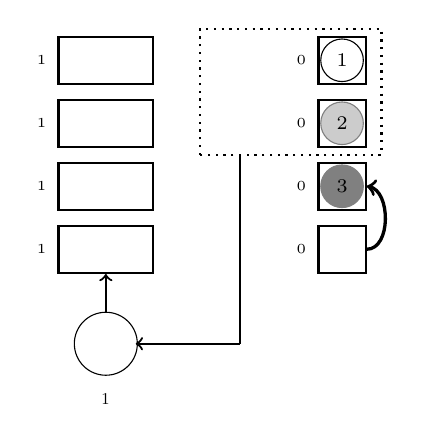
\begin{tikzpicture}
[
textbox/.style={rectangle, draw=white, fill=white,align=center, thick, minimum height=0.5cm},
box1/.style={rectangle, draw=black, fill=white, thick, minimum height=0.6cm, minimum width=2.4cm},
box2/.style={rectangle, draw=black, fill=white, thick, minimum height=0.6cm, minimum width=1.2cm},
box3/.style={rectangle, draw=black, fill=white, thick, minimum height=0.6cm, minimum width=0.6cm},
buf/.style={rectangle, draw=black, fill=white, very thick, minimum height=0.6cm, minimum width=1.2cm},
myarrow1/.style={single arrow, draw=black, fill=black, 
      minimum width = 1mm, single arrow head extend=1mm,
      minimum height=1cm},
myarrow2/.style={single arrow, draw=black, fill=red, 
      minimum width = 1mm, single arrow head extend=1mm,
      minimum height=1.3cm},
myarrow3/.style={single arrow, draw=blue, fill=blue, 
minimum width = 0.09cm, single arrow head extend=0.05cm,
minimum height=0.7cm},
mylabels/.style={text=black, font=\scriptsize},
    every label/.append style={mylabels},
    greenball/.style={circle, draw=gray, fill=gray!40, minimum size=1mm},
redball/.style={circle, draw=black, fill=white, minimum size=1mm},
blueball/.style={circle, draw=gray, fill=gray, minimum size=1mm},
]
\node at (0,0) [box2,label={west:$\OLDEST_1$}] (b10)  {};
\node at (0,-0.8) [box2,label={west:$\OLDER_1$}] (b11)   {};
\node at (0,-1.6) [box2,label={west:$\OLD_1$}] (b12)  {};
\node at (0,-2.4) [box2,label={west:$\NEW_1$}] (b13)  {};


\node[scale=0.6] at (0,-4.3) [textbox] (omap1) {\Large{$\omerge_1$}};
\draw[] (0,-3.6) circle (4mm) node (c2)  {};
\draw[color=black,thick,->]  (0,-3.2) -- (b13) {};
\draw[color=black,thick] (1.7,-1.2) -- (1.7,-3.6) {};
\draw[color=black,thick,->]  (1.7,-3.6) -- (0.38,-3.6) {};
\node at (3,0) [box3,label={west:$\OLDEST_0$}] (b10) {};
\node at (3,-0.8) [box3,label={west:$\OLDER_0$}] (b11)  {};
\node at (3,0) [redball] (g1) {{\scriptsize 1}};
\node at (3,-1.6) [box3,label={west:$\OLD_0$}] (b12)  {};
\node at (3,-0.8) [greenball] (g2) {{\scriptsize 2}};
\node at (3,-2.4) [box3,label={west:$\NEW_0$}] (b13)  {};
\node at (3,-1.6) [blueball] (g2) {{\scriptsize 3}};
\draw[dotted,color=black,thick] (1.2,-1.2) rectangle (3.5,0.4);
\draw [->,color=black!50!black,very thick] (b13.east) to [out=0,in=-10] (b12.east) ;
\end{tikzpicture}
%\caption{}
\end{subfigure}
}
%\caption{\LSDd[$\cdot$]: from $\Sigma$ to DSE.(a) Insertion of the 1st entry happens at $\NEW_0$(Rule 1), making $\NEW_0$ full. Hence it is moved to the empty old index $\OLDEST_0$ (Rule 2, red arrow). The 2nd insertion happens at $\NEW_0$ (Rule 1), making it full again, and is moved to next empty old index $\OLDER_0$ (Rule 2, dark red arrow).(b) During the 3rd insertion, both $\OLDEST_0$ and $\OLDER_0$ are full, so the next $\gamma$ steps of $\Sigma.$\omerge$_1$\ is called (Rule 3), moving entries from $\OLDEST_0\cup \OLDER_1$ (directly or via a buffer) to $\NEW_0$ in the next $2^1$ steps. The 3rd entry is inserted at $\NEW_0$ and moved to $\OLD_0$ (triggering Rule 1 and 2 respectively). (c) During the 4th insertion, $\OLDEST_0$ and $\OLDER_0$ are still full, hence next $\gamma$ steps of $\Sigma.$\omerge (Rule 3) is called. At this point $2^1$ steps of \omerge$_1$\ are done and $\NEW_1$ is full with entries of $\OLDEST_0\cup \OLDER_1$, and is moved to $\OLDEST_1$ (Rule 2, light red arrow). The 4th insertion causes $\NEW_0$ to be full. Hence $\OLD_0$ is moved to $\OLDEST_0$ (red arrow), and $\NEW_0$ is moved to $\OLDER_0$(dark red arrow).}
\label{fig:sddFig}
\end{figure}
	

\begin{figure*}[!h]
\begin{mdframed}
\begin{algorithmic}%[1]
 \Statex \hskip-1.5em$\Gamma \in \{\OneChoice,\TwoChoice, \NlogN \}$
\Statex \hskip-1.5em If $\Gamma = \OneChoice$, $N'= 3{\cdot} 2^i,m_i = \lceil{\frac{2^i}{\log 2^i \log \log 2^i}}\rceil$,  $\forall level\in \{0 \ldots m_i-1\}$ $b_{level} = 3{\cdot}\log 2^i\log \log 2^i$ and $c_{level} = 0$
\Statex \hskip-1.5em If $\Gamma = \NlogN$, $N'= 2^i{\cdot}\log{(2^i+1)}$, $m_i = (i+1)$,   $\forall level\in \{0 \ldots m_i-1\}$ $b_{level} = 2^{level}$ and $c_{level} = 2^{i-level}$
\Statex \hskip-1.5em If $\Gamma = \TwoChoice$, $N'= z{\cdot} 2^i,m_i = \lceil{\frac{2^i}{(\log \log 2^i) (\log \log \log 2^i)^2}}\rceil$,
$\forall level\in \{0 \ldots m_i-1\}$ $b_{level} = z{\cdot}(\log \log 2^i)(\log \log \log 2^i)^2$ and $c_{level} = 0$, $2 \leq z \leq 4$
\Statex
\end{algorithmic}
\underline {{${\sf NEW}_i$ $ \leftrightarrow$ {$\Gamma$.\omerge$_i(K, \sigma; {\sf OLDEST}_{i - 1},{\sf OLDER}_{i - 1})$}}}
\begin{algorithmic}[1]
\item[Client $\leftrightarrow$ Server:] %\tpurp{$\Gamma$ s inside the function should be deleted}
\Statex
\Statex \textcolor{blue}{//** \ \ Phase 1 - Preparing sorted input array\ \   **//}	
\State Client parses $K$ as $(k_{rnd},P)$ \label{fw:parseK}\Comment{all encryptions and decryptions are done with key $k_{rnd}$, $P$ is an array of PRF keys}
%\State Client initializes a tuple called $\pr$ as $(\bot, 0)$ and stores it in local state $\sigma$
\State {Server initializes} arrays \BUF$_1$ of size $3{\cdot}N'$, and \BUF$_2$ of size $N'$ to be empty at Server\label{fw:init}
%\State Perform oblivious sort on $\OLDEST_{i-1}.\Ind \cup \OLDER_{i-1}.\Ind$ in 
%the lexicographic order of keywords; store output in $\BUF_1$ \label{fw:firstsort}
\State Copy $\OLDEST_{i-1}.\Ind \cup \OLDER_{i-1}.\Ind$ to $\BUF_1$; obliviously sort $\BUF_1$ w.r.t. 
 lexicographic order of keywords\label{fw:firstsort}
\State Perform two linear scans (one in reverse and one in correct order) on $\BUF_1$, to add the $rank$ and $n_w$ values to each entry of keyword $w$. The entries now look like $(w,id,op,rank,n_w)$, where $0 \leq rank < n_w$. \label{fw:twoscans}
\State {Linearly scan $\BUF_1$ and pad each keyword-list with dummy elements so that its size is nearest power of 2, hide list lengths by padding total size to $2N'$}\label{fw:pad2}% without leaking the actual list length}
   % \State {$cnt \gets 0$}
   \State {Perform oblivious sort on $\BUF_1$ w.r.t. lexicographic order of the keywords and descending order of the $n_w$ values. Keep first $N'$ elements.}\label{fw:secondsort}
   \Statex
  \Statex \textcolor{blue}{//** \ \ Phase 2---Prepare index elements and prepare keyword counters \ \ **//}	
    \For{each $j = 1 \ldots |\BUF_1|$}\label{fw:loop1start}
    \State Client decrypts $(w,id,op,rank,n_w) \gets \RND.\Dec(k_{rnd},\BUF_1[j])$\label{fw:dec1} %
      \State Client generates {$p \gets^{\$} \{0,1\}^\lambda$}\label{fw:randp}
    \IIf{$rank = 0$}{~Client appends $(\RND.\Enc(k_{rnd},(w,n_w,p)))$ to $\BUF_2$}\label{fw:rank0} %\Comment{\tpurp{I want to do p+1 here}}
    \ElsI{Client appends $(\RND.\Enc(k_{rnd},(\bot,\bot,\bot)))$ to $\BUF_2$}\label{fw:rankN0}
    \State Client generates $((level,pos),\sigma)\gets\texttt{Map}(P[i][3],w,rank,n_w,\sigma)$\label{fw:map} \Comment{$pos=0$ for \OneChoice\ and \TwoChoice\ }
  \State Client writes $(\RND.\Enc(k_{rnd},(w,id,op,level,pos)))$ to \BUF$_{1}[j]$ \label{fw:dec2}
    \EndFor\label{fw:loop1end}
    \Statex
    \Statex \textcolor{blue}{//** \ \ Phase 3---Add dummies\ \ **//}	%\Comment{this phase adds binsize dummy entries per bin}
    \For{$level= 0 \ldots m_i-1$}\label{fw:loop2start}
    \State for every $pos \in\{0 \ldots c_{level}\}$ call Client appends $(\RND.\Enc(k_{rnd},(\bot,\bot,\bot,level,pos)))$ to $\BUF_1$  $b_{level}$ times \label{fw:padbin}
    \EndFor\label{fw:loop2end}
    \Statex
     \Statex \textcolor{blue}{//** \ \ Phase 4---Final placement \ \ **//}	
    \State Perform oblivious sort on $\BUF_1$ w.r.t. the integer values of $(level,pos)$ in ascending order \label{fw:thirdsort}
    \State Linearly scan $\BUF_1$, and tag \textbf{first} $b_{level}$ entries for each $level\in \{0, \ldots, \Sigma.m_i-1\}$ and $pos\in \{0, \ldots, c_{level}\}$ with 1, and with 0 the rest of them (the existing $(level,pos)$ tags are replaced with 0/1 tags, the entries now look like $(w,id,op,x)$, where $x \in \{0,1\}$)\label{fw:0-1tag}
    \State {Perform order preserving oblivious compaction on $\BUF_1$; keep first $N'$ entries; discard the 0/1 tags }\label{fw:compaction}
    \State Perform oblivious sort on $\BUF_2$ w.r.t. the random keys in ascending order; keep first $2^i$ entries; discard random keys\label{fw:buf2sort}
    \State 	Server moves $\BUF_1$ to \NEW$_i.\Ind$  \label{fw:newi} \Comment{elements in each $bin/pos$ is randomly shuffled}
   \For{each $s \in \BUF_2$}\label{fw:dictloopstart}
\State Client decrypts $(w, cnt_w) \gets \RND.\Dec(k_{rnd}, s)$\label{fw:dec3}
\State Client generates $(key,value) \gets \PiBas.\MAP((P[i][3],k_{rnd}),w,cnt_w,1)$ \label{fw:pibasmap}\Comment{parameter 1 is used by the PRF $F$}
\State 	Client writes \NEW$_i.$\Dict[$key$] $\gets value$\label{fw:mapdict}
\EndFor\label{fw:dictloopend}
%\Statex
\State \Return \NEW$_i$
\end{algorithmic}
\end{mdframed}
%\vspace{-1.2em}
\caption{\omerge\ framework of $\Gamma \in \{\OneChoice, \TwoChoice, \NlogN\}$}
\label{alg:framework}
\vspace{+1.3em}
\end{figure*}

\smallskip\noindent\textbf{Phases of {\omerge} framework.}\label{sec:oblivious_merge}
%\todo{5.Clearly explain that SDd[] works only with 1C/2C/NlogN and not scheme-agnostic}
Now we will present our \omerge\ framework that 
ensures properties \textsf{{(P1)}}, \textsf{{(P2)}}, 
and \textsf{{(P3)}} for the static 
SE scheme $\Gamma$ $\in$ $\{\OneChoice,$ $\TwoChoice,$ $\NlogN\}$, in detail. 
%\todo{7.Clarify which scheme targets which storage and which metrices} 
Similar to \SDa, we have \LSDd[\OneChoice] and \LSDd[\TwoChoice] (suitable for HDDs), as well as \LSDd[\NlogN] (compatible with both HDDs and SSDs).
The corresponding is presented in Figure \ref{alg:framework}. 
Some of the steps are not necessary for all the schemes in  $\{\OneChoice,$ $\TwoChoice,$ $\NlogN\}$, 
but we needed them in order to create the general \omerge\ framework. 
\new{Towards the end of this section we discuss some optimization specific to each scheme.  Here, we also would like to point out, the temporary client storage cost is upper bounded by the update cost (e.g. $\bO(\log^2 N)$ for \LSDd[\OneChoice]), while the permanent client storage is constant. }

The high level idea is, instead of moving elements directly from 
$\OLDER_{i-1}.\Ind \cup \OLDEST_{i-1}.\Ind$ to $\NEW_i.\Ind$ 
(using oblivious dictionaries, as done in \cite{SDa}), 
move them to a buffer $\BUF_1$ first. This step will ensure 
property \textsf{{(P2)}}. Then with oblivious operations, re-order the entries of $\BUF_1$ to 
satisfy the I/O efficiency requirements of scheme $\Gamma$, 
and then move $\BUF_1$ to $\NEW_i$.\Ind. {This step and the previous step 
together ensure property \textsf{{(P1)}}. 
{The buffer, $\BUF_2$, is used to create  
the keyword dictionary, $\NEW_i.\Dict$}, in an oblivious fashion as well.
The references to $\OLDER_{i-1}$ and $\OLDEST_{i-1}$ are passed as parameters to the \omerge$_i$ protocol.
Each \omerge$_i$ instance runs in four phases. Below we discuss the four phases in detail. Refer to Figure \ref{alg:framework} for the pseudocode. 
If a step in the pseudocode does not mention who is performing it (i.e. Client or Server), it means multiple rounds of communication happens between the client and the server to perform that step.}
\neww{Finally, at the end of $2^i$ calls to \omerge$_i$ it returns $\NEW_i$ (i.e. $\NEW_i.\Ind$  and $\NEW_i.\Dict$). }

\noindent\textbf{\underline{Phase 1.}} %In this phase 
\new{Entries of $\OLDER_{i-1}.\Ind \cup \OLDEST_{i-1}.\Ind$ are 
first copied (not moved) to $\BUF_1$.} Next, $\BUF_1$ is 
obliviously sorted based on the lexicographic order 
of the keywords (line \ref{fw:firstsort}). \new{The sort places 
entries for the same keyword adjacent to each other in $\BUF_1$, 
and the dummy entries are placed at the end. Each entry of 
$\BUF_1$ is then assigned a $rank$} and an $n_w$ value via two 
linear scans (line \ref{fw:twoscans}). Next, each keyword-list 
in $\BUF_1$ is padded to make their lengths to be nearest power of 2 
(line \ref{fw:pad2}). Another oblivious sort is performed on $\BUF_1$, 
based on the lexicographic order of the keywords, as well as descending 
order of the $n_w$ values   (line \ref{fw:secondsort}). This sort places 
same keyword entries adjacent to each other and entries with higher 
$n_w$ values are placed before entries with lower $n_w$ values in $\BUF_1$.

We provide a more detailed pseudocode for lines \ref{fw:twoscans} and \ref{fw:pad2} in the extended version.

\noindent\textbf{\underline{Phase 2.}} This phase prepares the elements in $\BUF_1$ for 
$\NEW_i.\Ind$ by adding proper position tags to them 
(lines \ref{fw:map}-\ref{fw:dec2}), and prepares $\BUF_2$ 
for creating $\NEW_i.\Dict$ (lines \ref{fw:randp}-\ref{fw:rankN0}). 
For every entry in $\BUF_1$\ $(w,id,op,rank,n_w)$ an entry is appended to 
$\BUF_2$. When $rank=0$, a real entry $(w,n_w,p)$ 
is appended to $\BUF_2$. 
\new{In all other cases a dummy entry $(\bot,\bot,\bot)$ is added (line \ref{fw:rankN0})
(because we can neither reveal the length of each keyword-list, nor the number of unique keywords). }
Here, $p$ is a uniformly generated random key of $\lambda$ bit.

The $\MAP$ function of $\Gamma$ is called for each 
entry of $\BUF_1$,  which %with appropriate arguments, which 
returns a pair $(level,pos)$. 

 \new{For every $\Gamma \in \{\OneChoice,\TwoChoice,\NlogN\}$ the pseudocode for the corresponding $\MAP$ function is provided in the extended version}.
For $\OneChoice$ and $\TwoChoice$ the value of $level$ indicates  
the bin number assigned to this entry, and $pos$ is 0 by default. 
Whereas, for \NlogN\ scheme 
$level(\in \{0,\ldots,i\})$ indicates the array level,
and position indicates the position $pos (\in \{0,\ldots, (2^{i-level}\minus1)\})$ in the array level.
The encrypted entry $(w,id,op,level,pos)$ replaces the existing 
$(w,id,op,rank,n_w)$ entry in $\BUF_1$. 

\noindent\textbf{\underline{Phase 3.}}
This phase adds dummy elements 
(lines \ref{fw:loop2start}-\ref{fw:loop2end}) to $\BUF_1$, beacuse  
every bin needs to be filled up to their maximum capacity. 
For \OneChoice\ and \TwoChoice\, if bin size is $b_i$ then 
the dummy element $(\bot,\bot,\bot,bin,0)$ is appended to $\BUF_1$ $b_i$ times. 
This step is repeated for each bin number $bin$.  
For \NlogN\ scheme, array level $k$ contains $2^{i-k}$ 
lists of size $2^k$.
Hence, the dummy entry $(\bot,\bot,\bot,k,pos)$ 
is appended $2^k$ times for each $pos \in \{0,\ldots, (2^{i-k}-1)\}$.
This step is repeated for levels $k \in \{0, \ldots, i\}$. 
\new{We add a total of $3{\cdot}2^i$ dummy elements for \OneChoice\ and 
\TwoChoice\, and $2^i{\cdot}\log {2^i}$ dummy elements for \NlogN.
The goal is to add dummy entries for every vacant positions of the bins/levels.
But we want} to hide the number of real elements {in each bin/level, and so 
 the number of dummy elements we add is equal to the index size.
Extra dummy elements are discarded in Phase 4.}
\noindent\textbf{\underline{Phase 4.}} 
This phase consists of few steps. 
%(lines \ref{fw:thirdsort}-\ref{fw:dictloopend}). 
%Each of them can be de-amortized.
The oblivious sort on line \ref{fw:thirdsort} 
sorts $\BUF_1$ based on $(level,pos)$ values.
Dummy elements come last, as usual.
But now we have more elements assigned to each bin/level than their capacity. 
Hence, with a linear scan (line \ref{fw:0-1tag}) 
unnecessary elements are tagged with a 0;
and the entries to be kept are tagged with a 1. 
%(red and blue tags respectively in Figure \ref{fig:buf1f}).
This tag replaces the existing $(level,pos)$ tags.
Next, an order preserving oblivious compaction (line \ref{fw:compaction}) is 
performed so that all elements tagged with 0 come at the tail of the output and 
can be discarded altogether. We use 
another round of oblivious bucket sort (which is order preserving) for the compaction. 
%The 0/1-bit tags are removed from each entry at the end.
%Next, the entries %at the beginning that were tagged with 
%1-bit in 
$\NEW_i.\Ind$ is created with the remaining entries of $\BUF_1$ (line \ref{fw:newi}). 
$\BUF_2$ is also obliviously sorted (line \ref{fw:buf2sort}) based on 
the random keys in ascending order. 
The dummy entries with $p=\bot$ will be placed at the end of the sorted buffer.
There can be at most $2^i$ entries such that $p \neq \bot$, as 
there can be at most $2^i$ distinct keywords at index level $i$.
Hence, the first $2^i$ elements are used to 
create $\NEW_i.\Dict$ (lines \ref{fw:dictloopstart}-\ref{fw:dictloopend}).

\smallskip\noindent\textbf{Locality-aware \LSDd$[\cdot]$.}
\new{The search-\emph{locality} and search-\emph{read efficiency} of \LSDd[$\Gamma$]
depends on the same of the static SE scheme $\Gamma$. For both \emph{locality} 
and \emph{read efficiency}, a $\log N$ factor is added 
due to querying $3{\cdot}\log N$ dictionaries and calling 
$\Gamma.\Search$ on $3{\cdot}\log N$ indexes (for \OLDEST, \OLDER, and \OLD). 
For example, \OneChoice\ offers $\bO(1)$ \emph{locality} 
and $\bO(\log N \log \log N)$ \emph{read efficiency}, whereas \LSDd[\OneChoice] offers 
$\bO(\log N)$ \emph{locality} and $\bO(\log N \log \log N +\log N)$ \emph{read efficiency}. 
Similarly, \LSDd[\NlogN] offers $\bO(\log N)$ \emph{locality} and $\bO(\log N)$ \emph{read efficiency}, 
as opposed to optimal \emph{locality} and \emph{read-efficiency} that is offered by \NlogN.} 

\smallskip\noindent\textbf{Page-efficient \LSDd{[.]}.}
We can instantiate \LSDd[$\cdot$] on SSDs with static page efficient schemes 
like \NlogN\  \cite{onechoice} and its variations i.e. \Ns\ \cite{Demertzis17}. 
The \emph{page efficiency} of \LSDd[\NlogN] is $\bO(\log N)$ vs. the 
optimal \emph{page efficiency} offered by \NlogN, whereas 
for \LSDd[\Ns] \emph{page efficiency} is $\bO(N^{\frac{1}{s}}/p+\log N)$. 

\smallskip\noindent\textbf{Security and efficiency.} We formally state and prove the security of \LSDd[$\Gamma$] 
(for $\Gamma \in \{\OneChoice,\TwoChoice,\NlogN\}$) in the extended version. The security of \SDd[\PiBas] is already proven in \cite{SDa}. 
We prove also that when we instantiate a locality-aware static scheme $\Gamma$ with \LSDd[$\cdot$], it retains its space overhead, but for \emph{locality} and \emph{read-efficiency} an additional $3\log N$ factor is introduced as $3\log N$ indexes are queried (similar proof for the \emph{page-efficient} \LSDd[$\cdot$] transformation can be proven)---see the extended version. 

\smallskip\noindent\textbf{\OneChoice\ Optimization.} 
In \OneChoice\ scheme we do not need to make the keyword-lists' sizes to be of power of 2. 
We also do not need to store the larger keyword-lists into the bins before the 
smaller lists. Hence the lines \ref{fw:pad2} and \ref{fw:secondsort} 
in Figure \ref{alg:framework} are not required for \OneChoice.
%In Figure \ref{alg:sdd1C} those two lines are omitted.
The two linear scans that add $rank$ and
$n_w$ values to each entry can be also removed (line \ref{fw:twoscans}). 
This is because, after the first oblivious sort
the entries for the same keyword are all placed together in adjacent locations. In Phase 2, with the help of a single counter 
%($cnt$ variable in 
%line \ref{sdd1c:counter} in Figure \ref{alg:sdd1C}), 
one can count how many occurrences of 
a particular keyword has been seen. %(and $\BUF_2$ can be updated accordingly).
Based on this counter value $\BUF_2$ can be updated accordingly.
The same counter value can be used in $\OneChoice.\MAP$ function to compute 
the bin numbers.% (line \ref{sdd1c:map} in Figure \ref{alg:sdd1C}).
The counter needs to be reset to 0 every time a new keyword is observed. We provide the optimized pseudocode for  \OneChoice.\omerge\ in the extended version. 


\smallskip\noindent\textbf{\NlogN\ Optimization.} 
%\paragraph{{\textbf{\NlogN\ Optimization.}}}
Here the order of storing lists does not matter.
Thus, the second oblivious sort (line \ref{fw:secondsort}) can be omitted in Phase 1 for the \NlogN\ scheme.
This can be further optimized 
by storing only $s$ evenly distributed arrays, 
instead of $\ell=\log N+1$ arrays, which 
is essentially the \textsf{Ns} scheme.

\smallskip\noindent\textbf{\TwoChoice\ Optimization.} 
For \TwoChoice\ scheme, the client needs to maintain a map to remember which bin has how many entries.
This is because, placement of a keyword-list into a superbin 
depends on how full the superbin is. 
There are can be maximum of $m = \lceil{{N}/{\log\log N (\log \log \log N)^2}}\rceil$  
bins. But in \LSDd\ there are $\log N$
index levels. Hence, to maintain this information the required  
client storage is $\bO(m{\cdot}\log N)$.
To achieve a constant client storage, this map can 
be stored at the server in oblivious maps (see section \ref{sec:prelim}).

\smallskip\noindent\textbf{Update cost.}
The \omerge\ framework shown in Figure \ref{alg:framework} mainly consists of three types of building blocks: bucket oblivious sorts, 
basic \algorithmicfor\ loops and linear scans.
Linear scans are realized with basic \algorithmicfor\ loops. 
The costliest operation among these is the bucket oblivious sort \cite{bucketSort}, 
which can be decomposed into $N$ steps of $\bO(\log N)$ work per step, 
assuming an index contains at most $N$ entries 
(recall the $i$th index contains $2^i$ elements).
In the extended version we explain how to 
deamortize the bucket oblivious sort in detail. 
Even the \algorithmicfor\ loops can be executed for $\bO(\log N)$ 
iterations during a particular call of \omerge$_i$ (for the $i$th index). Overall, an \omerge$_{i}$ protocol can be decomposed into $N$ steps of at most $\bO(\log N)$ work per step. There are $\log N$ levels in \LSDd[${\cdot}$]. Hence, the \emph{worst case} update cost is $\bO(\log^2 N)$ for \LSDd[\OneChoice], and \LSDd[\TwoChoice]. For \LSDd[\NlogN] the update cost is $\bO(\log^3 N)$, because it has at most $\log N$ levels per index.